\chapter{Tactile Perception} \label{ch:1-tactile-perception}

This chapter presents an analysis of the performance of a \gls{dl} model in simulating realistic tactile data, with a specific focus on its ability to simulate contact normals and skew forces. Contact normals are essential for accurately estimating the pose of an object in contact, while skew forces are critical for predicting the behavior of an object when it is grasped and manipulated by the Shadow Dexterous hand. \medskip

To estimate the contact normals, \gls{rls} is applied with estimated linear velocities. The performance of which is compared to the contact normals produced by Gazebo's physics engine, and the \gls{gt} normals.\medskip

The technique behind estimating the skew forces is a \gls{dl}, including its architecture, is described, and the methodology used to test the network is presented. The testing methodology involves the use of various input data, and the output is analyzed for accuracy and realism. The findings are presented and discussed, including the strengths and weaknesses of the network in simulating tactile data. Finally, an assessment is made of the network's ability to produce tactile data that is realistic. \medskip

The software used in this chapter is a regression neural network implemented as a Gazebo \texttt{ModelPlugin}~\cite{gazebo-model-plugin} in C++. However, the \gls{dl} model plugin used in the original publication~\cite{simulation-of-the-syntouch-biotac-sensor} has not been updated since 2018, making the code incompatible with the current version of Gazebo API. Moreover, the licensing issues with the files in the \texttt{xmlrpc++} library, which were used for base64 encoding and decoding, necessitated their removal~\cite{base64-encoding-decoding-licensing-issue}. To address these issues, each has been resolved and the plugin has been reorganized and repackaged for compatibility with the current version of Gazebo. The original version of the plugin can be found in~\cite{ruppel-philipp-biotac-gazebo-plugin}, while the fixed and updated version is available at~\cite{melbye-staven-biotac-sim-plugin}. \medskip

The availability of the updated plugin ensures that the project can continue to benefit from the capabilities of the \gls{mlp} based \gls{dl} model for simulating realistic tactile data in the current version of Gazebo.


\section{Method}\label{sec:1-tactile-perception-method}

\subsection{Recursive Least Squares} \label{sec:1-tactile-perception-recirsive-least-squares}




\subsection{Network Architecture}\label{sec:1-tactile-perception-method-network-architecture}
% wrap
In~\cite{simulation-of-the-syntouch-biotac-sensor} two different architectures were built, where architecture B is chosen due to its better greater accuracy and lower execution time. The network architecture B can be seen in~\figref{fig:dl-model-tactile-perception}. As inputs, the network takes one contact position \mvar{\vec{c} = \rvec{c_x, c_y,c_z}} along with three force vector samples \mvar{\vec{f}_{1}=\rvec{f_{1,x},f_{1,y},f_{1,z}}}, \mvar{\vec{f}_{2}=\rvec{f_{2,x},f_{2,y},f_{2,z}}} and \mvar{\vec{f}_{3}=\rvec{f_{3,x},f_{3,y},f_{3,z}}}, and a temperature input \mvar{T\inR{}}, which makes the input \mvar{\rvec{\vec{c},\vec{f}_1,\vec{f}_2,\vec{f}_3,T}\inR{13}}. The outputs of the network are the data format produced by the physical sensor i.e. an output vector of \mvar{\rvec{pdc, pac, tdc, tac, e_1, \dots, e_{19}}\inR{23}}, where \mvar{pdc} is the pressure DC signal, \mvar{pac} is the pressure AC signal, \mvar{tdc} is the temperature DC signal, \mvar{tac} is the temperature AC signal and \mvar{e_1} to \mvar{e_{19}} are the electrode activations.

The network architecture consists of four \gls{mlp}s, one for interpreting the position input, one for interpreting the force inputs, one for interpreting the temperature input, and one for combining the interpretations of force and position inputs. \gls{mlp} \num{1}, responsible for interpreting the position data, consists of four hidden layers, three of which contain \num{512} neurons and uses \gls{relu} as the activation function, while the fourth and last uses a linear activation function with \num{64} neurons. The activation functions can be seen marked red if they use \gls{relu}, green if they use a linear activation function and blue if they use a sigmoid activation function. \medskip

\gls{mlp} \num{2} interprets the force inputs but rather than using \num{512}, uses \num{256} for its hidden layers, while still having the linear activation function and the \num{64} neurons in its fourth layer. This \gls{mlp} further differs as the \num{256} neuron layers apply \mvar{\ell_1} bias regularization. \gls{mlp} \num{3} produces a temperature correction vector using two hidden layers, one with \num{256} neurons and a sigmoid activation function and one with \num{23} neurons and a linear activation function. The last \gls{mlp}, \gls{mlp} \num{4} takes in the element-wise product of \gls{mlp} \num{1} and \num{2}, parses the product through two \num{256} neuron layers with \gls{relu} and one \num{23} neuron layer with a linear activation function.\medskip

The products of \gls{mlp} \num{3} and \num{4} are summed and parsed as the model's output.


% which is incorporated to achieve the final output vector. The temperature correction vector, comprising a densely connected layer of 256 neurons with sigmoid activation for smooth temperature regression and a reduction layer with linear activation, set to output size.

% The position and force inputs are handled by two distinct \gls{mlp}s, each comprising three densely connected layers with \gls{relu} activation. To enable accurate differentiation between various areas on the sensor surface, the position column employs \num{512} neurons per layer, whereas the force column employs \num{256} neurons per layer with \mvar{\ell_1} bias regularization. 

% Both columns conclude with a smaller output layer of 64 neurons with linear activation. The outputs of the position and force columns are multiplied together, and the product is processed through two densely connected layers with ReLU activation, each containing 256 neurons. The result is then reduced to output size by a smaller densely connected layer with linear activation. Finally, a temperature correction vector is incorporated to achieve the final output vector. The temperature correction vector is created by a third column, comprising a densely connected layer of 256 neurons with sigmoid activation for smooth temperature regression and a reduction layer with linear activation, set to output size.

% Initially, a densely connected sequential model (referred to as Network A) was developed, with five hidden layers of sizes 1024, 4096, 512, 512, and 512 and a ReLU activation function. Various experiments with different layer sizes, counts, and activation functions were conducted before settling on this configuration.

\begin{figure}[h]
		\begin{center}
			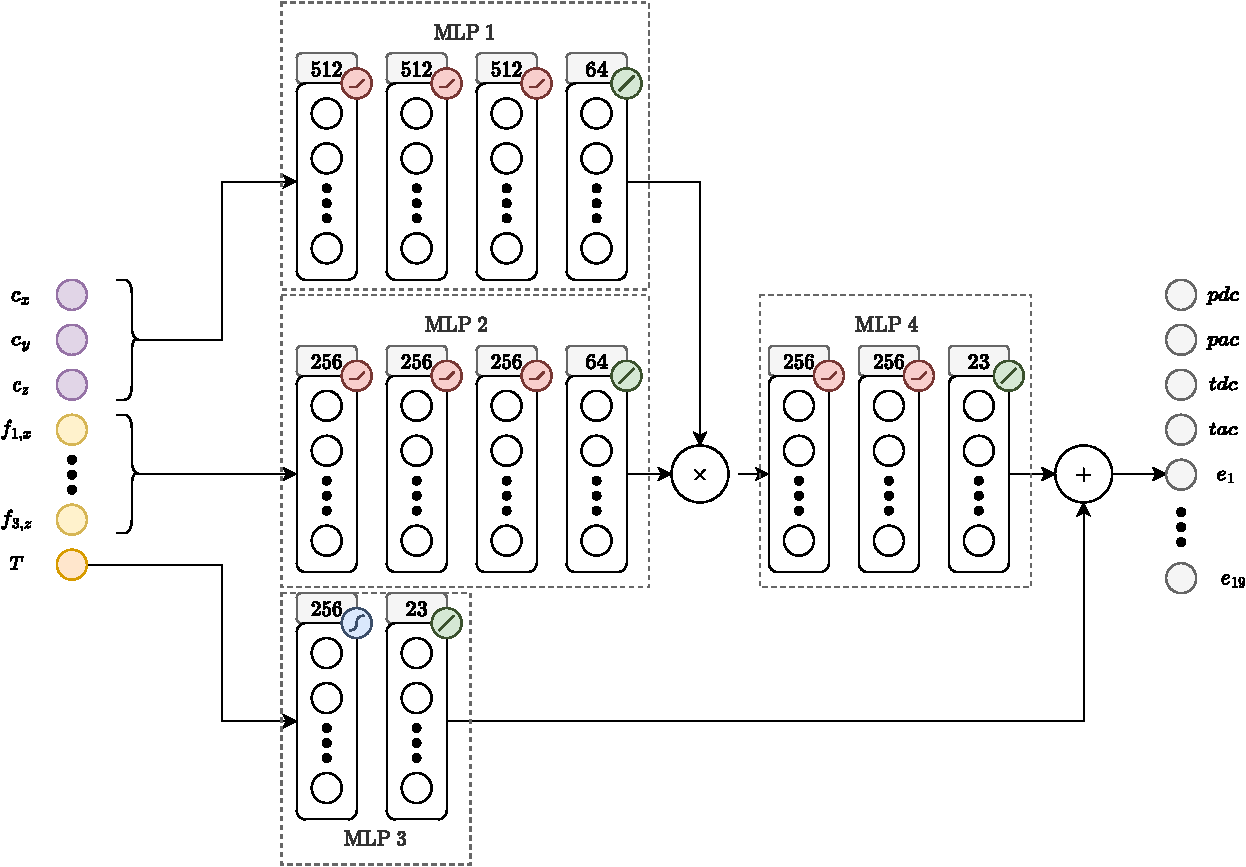
\includegraphics[width=\textwidth]{chapters/1-tactile-perception/fig/dl-model-tactile-perception-grouping-crop.pdf}
		\end{center}
		\caption{\gls{dl} model B from~\cite{simulation-of-the-syntouch-biotac-sensor}, which also has provided inspiration for this illustration.}
		\label{fig:dl-model-tactile-perception}
\end{figure}


\subsection{Network Training Procedure}\label{sec:1-tactile-perception-method-network-training-procedure}

The model presented in~\secref{sec:1-tactile-perception-method-network-architecture} was trained using a custom dataset collected by the authors. The dataset \mvar{D} contains \mvar{N_{dp} = \num{300 000}} tactile sensor readings, consisting of the complete BioTac sensor data as well as the applied reference forces. This can be seen below

\begin{equation} \label{eq:dl-data-matrix}
	D =
	\left[\begin{array}{@{}c|cccccccccccccc@{}}
		0       & pcd & pac & tdc & tac & e_{1} & \cdots & e_{19} & f_{1,x} & \cdots & f_{3,z} & c_x & c_y & c_z \\
		1       & pcd & pac & tdc & tac & e_{1} & \cdots & e_{19} & f_{1,x} & \cdots & f_{3,z} & c_x & c_y & c_z \\
		\vdots  &  &  &  &  &  &  & \vdots &  &  &  &  &  &  \\
		N_{dp}  & pcd & pac & tdc & tac & e_{1} & \cdots & e_{19} & f_{1,x} & \cdots & f_{3,z} & c_x & c_y & c_z
		\end{array}\right] \inR{N_{dp} \times 35}
\end{equation}

All inputs are normalized to have zero mean and unit variance, based on the distribution of the captured data. The three force vectors are sampled at intervals of \SI{100}{\milli\second} to prevent overfitting and avoid unrealistic reactions to high-frequency inputs that the physics simulator cannot replicate. The BioTac sensor electrode values exhibit a non-linear dependence on device temperature and attempts to correct this before inputting the data resulted in poor performance. Instead, the network was trained to compensate for this dependency by itself. During simulation, a constant temperature was assumed, which is typically the average temperature of the training set. The network generates simulated electrode and pressure signals as outputs but does not currently simulate temperature outputs. \medskip

The forces were collected using a calibrated six-axis force-torque sensor~\cite{ati:-6-axis-force-and-torque-sensor-nano17-series} with a nominal force resolution better than \SI{0.01}{\newton}. 

The contact position is reconstructed optically using a calibrated HD webcam and two AprilTag markers~\cite{apriltag:-a-robust-and-flexible-visual-fiducial-system}, one mounted on the BioTac and one attached to the probe object. The setup for this can be seen in \figref{fig:biotac-sim-experimental-setup}. Once the contact positions were collected, optimization-based calibrations were made to gain more accurate position estimates.

\begin{figure}[h]
	\begin{center}
		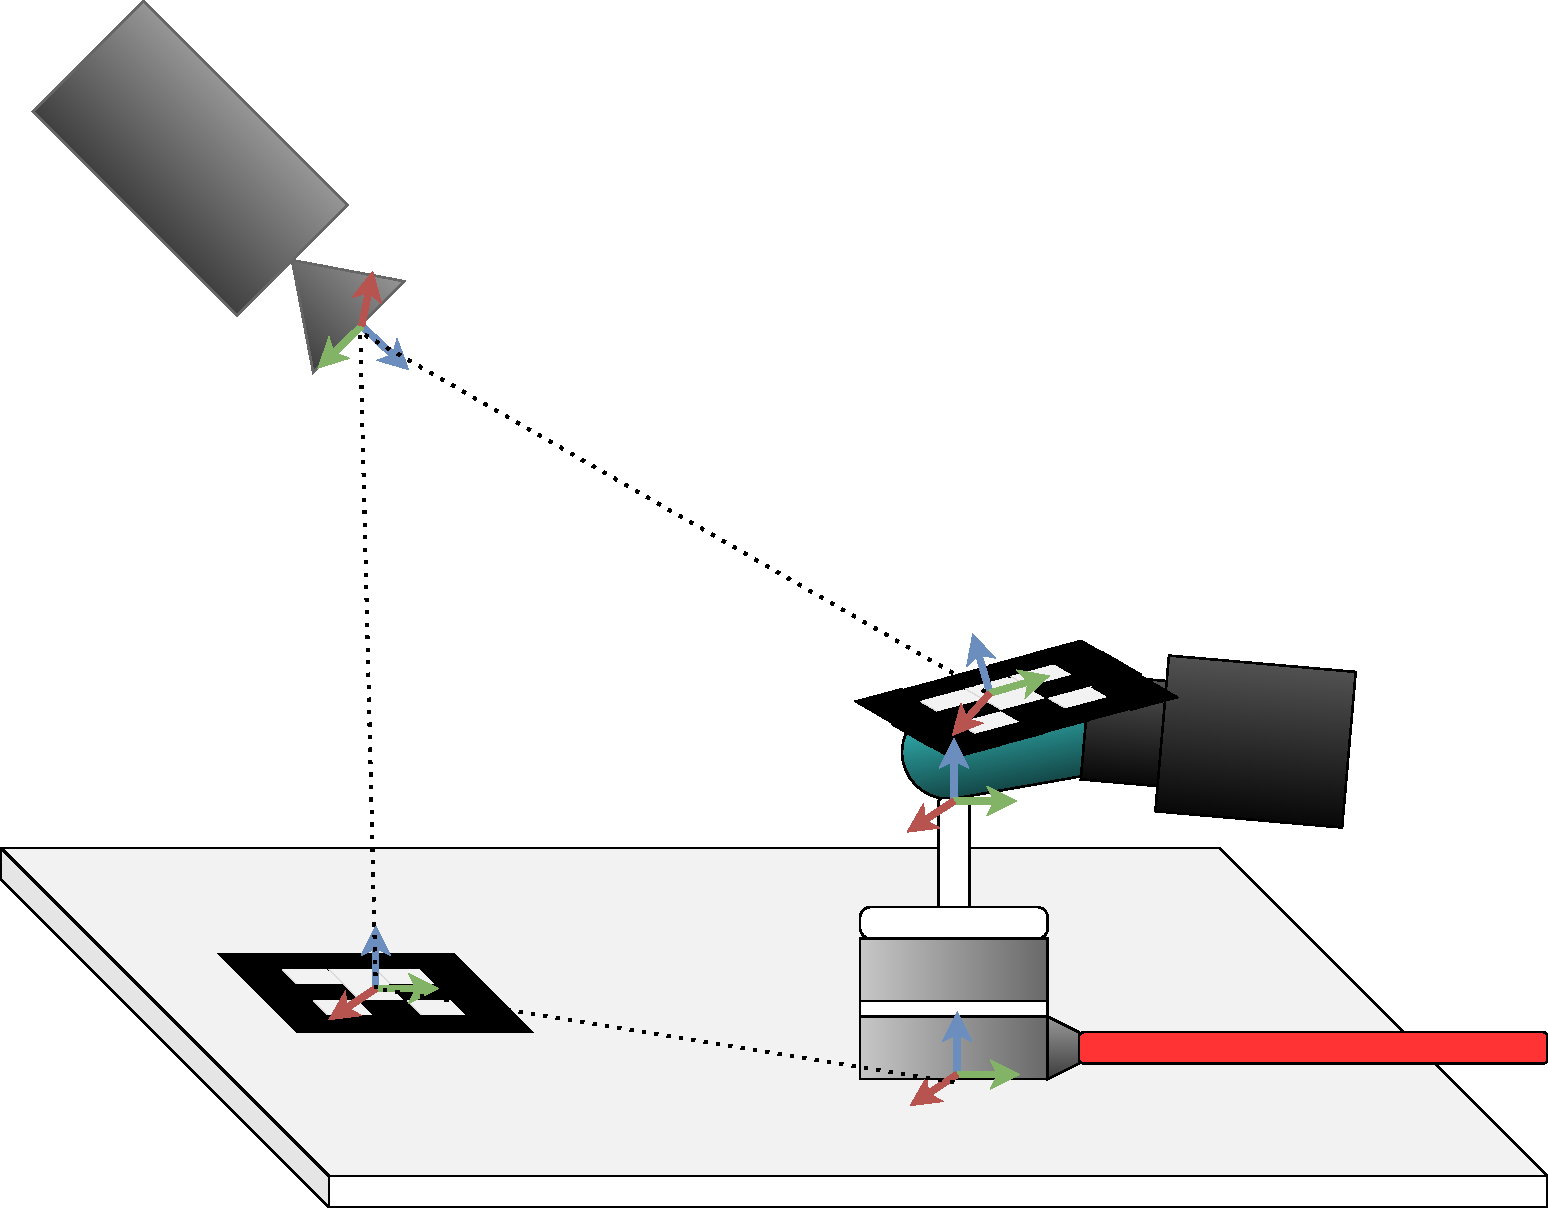
\includegraphics[width=0.7\textwidth]{chapters/1-tactile-perception/fig/biotac-sim-experimental-setup.pdf}
	\end{center}
	\caption{Experimental setup for gathering data to train \gls{dl} model B, as inspired by~\cite{simulation-of-the-syntouch-biotac-sensor}.}
	\label{fig:biotac-sim-experimental-setup}
\end{figure}

\section{Experimental Setup}\label{sec:1-tactile-perception-experimental-setup}

To test the performance of the \gls{dl} model, four objects surfaces were used with known normals. These can be seen in~\figref{fig:experimental-setup-tactile-perception} as a flat surface, an edge, a smooth surface and a corner.

\begin{figure}[h]
	\centering
	\begin{subfigure}[b]{0.24\textwidth}
		\centering
		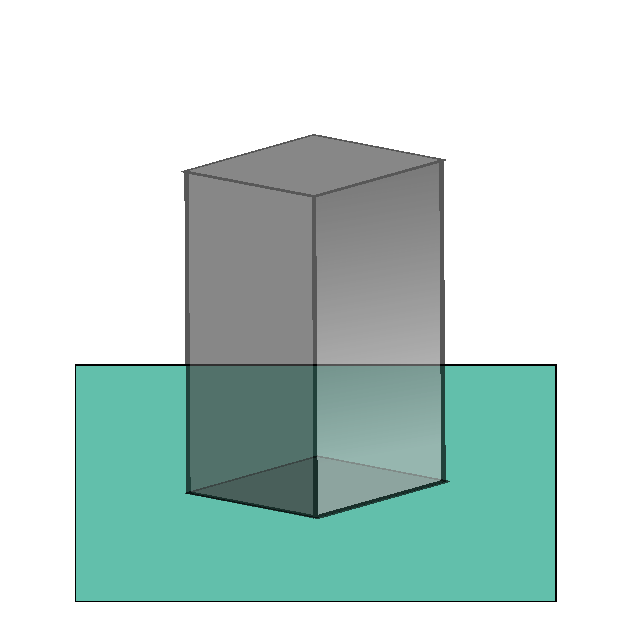
\includegraphics[width=\textwidth]{chapters/1-tactile-perception/fig/experimental-setup/flat-contact-3d.pdf}
		\caption{Finger in contact with a flat surface.}
		\label{fig:flat-contact}
	\end{subfigure}
	\hfill
	\begin{subfigure}[b]{0.24\textwidth}
		\centering
		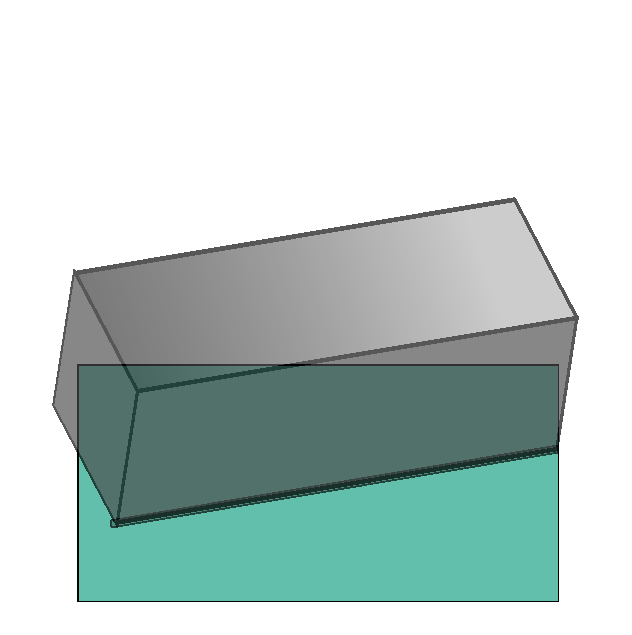
\includegraphics[width=\textwidth]{chapters/1-tactile-perception/fig/experimental-setup/edge-contact-3d.pdf}
		\caption{Finger in contact with an edge. \newline}
		\label{fig:edge-contact}
	\end{subfigure}
	\hfill
	\begin{subfigure}[b]{0.24\textwidth}
		\centering
		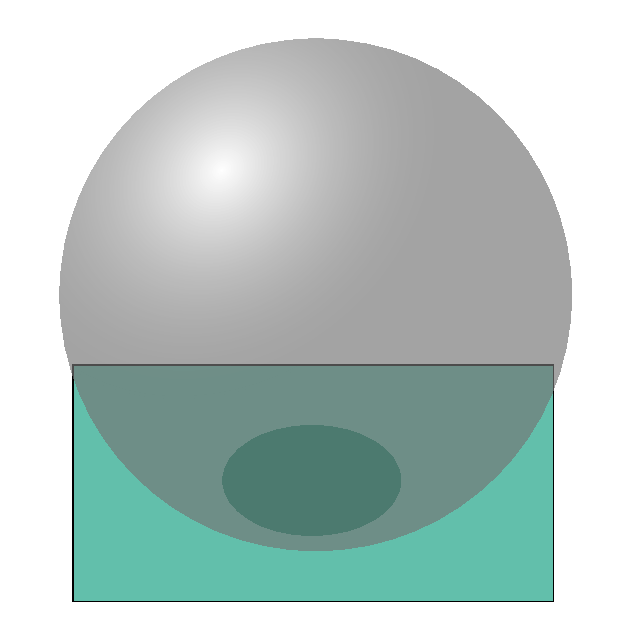
\includegraphics[width=\textwidth]{chapters/1-tactile-perception/fig/experimental-setup/smooth-contact-3d.pdf}
		\caption{Finger in contact with a smooth surface.}
		\label{fig:smooth-contact}
	\end{subfigure}
	\hfill
	\begin{subfigure}[b]{0.24\textwidth}
		\centering
		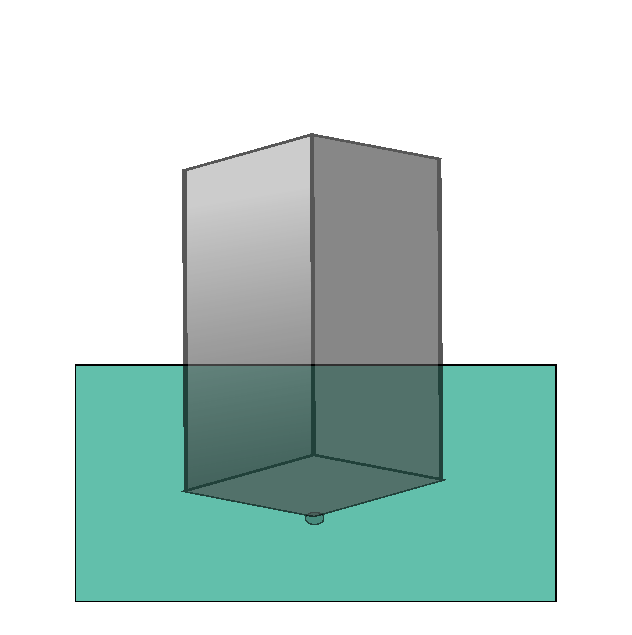
\includegraphics[width=\textwidth]{chapters/1-tactile-perception/fig/experimental-setup/corner-contact-3d.pdf}
		\caption{Finger in contact with a corner.\newline}
		\label{fig:corner-contact}
	\end{subfigure}
		\caption{The four surfaces used to test the performance of the \gls{dl} model's ability to represent surfaces.}
		\label{fig:experimental-setup-tactile-perception}
\end{figure}

Within the simulation, the index finger is set to make contact with each surface, as shown in~\figref{fig:experimental-setup-tactile-perception-experimental}.
\begin{figure}[h]
	\centering
	\begin{subfigure}[b]{0.24\textwidth}
		\centering
		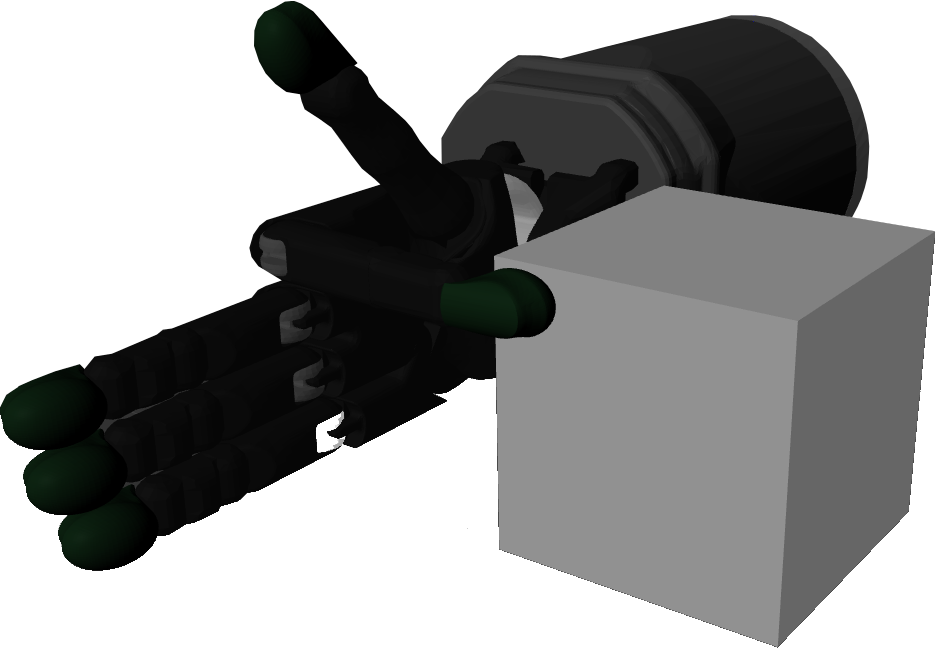
\includegraphics[width=\textwidth]{chapters/1-tactile-perception/fig/experimental-setup/flat-contact-crop.png}
		\caption{Simulated index finger in contact with a flat surface.}
		\label{fig:flat-contact-experimental}
	\end{subfigure}
	\hfill
	\begin{subfigure}[b]{0.24\textwidth}
		\centering
		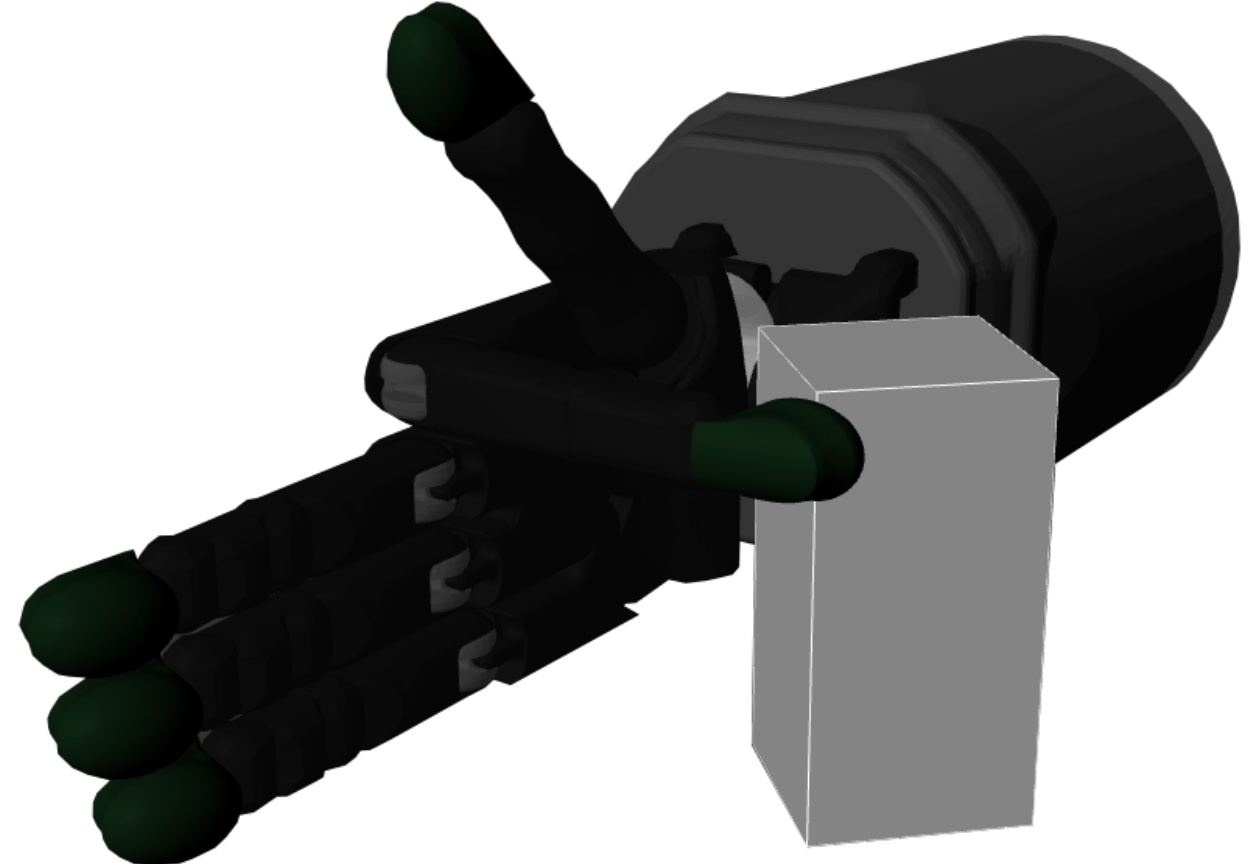
\includegraphics[width=\textwidth]{chapters/1-tactile-perception/fig/experimental-setup/edge-contact.png}
		\caption{Simulated index finger in contact with an edge.}
		\label{fig:edge-contact-experimental}
	\end{subfigure}
	\hfill
	\begin{subfigure}[b]{0.24\textwidth}
		\centering
		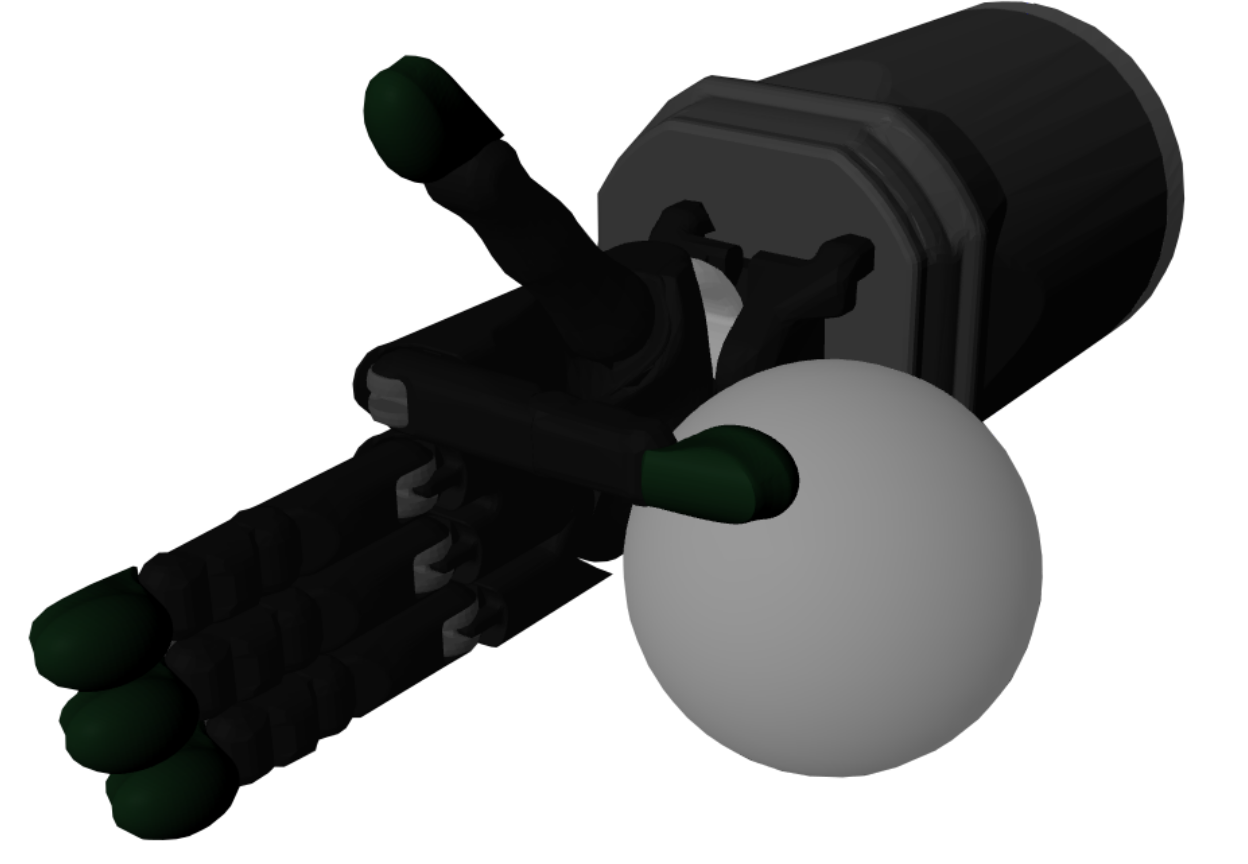
\includegraphics[width=\textwidth]{chapters/1-tactile-perception/fig/experimental-setup/smooth-contact.png}
		\caption{simulated index finger in contact with a smooth surface.}
		\label{fig:smooth-contact-experimental}
	\end{subfigure}
	\hfill
	\begin{subfigure}[b]{0.24\textwidth}
		\centering
		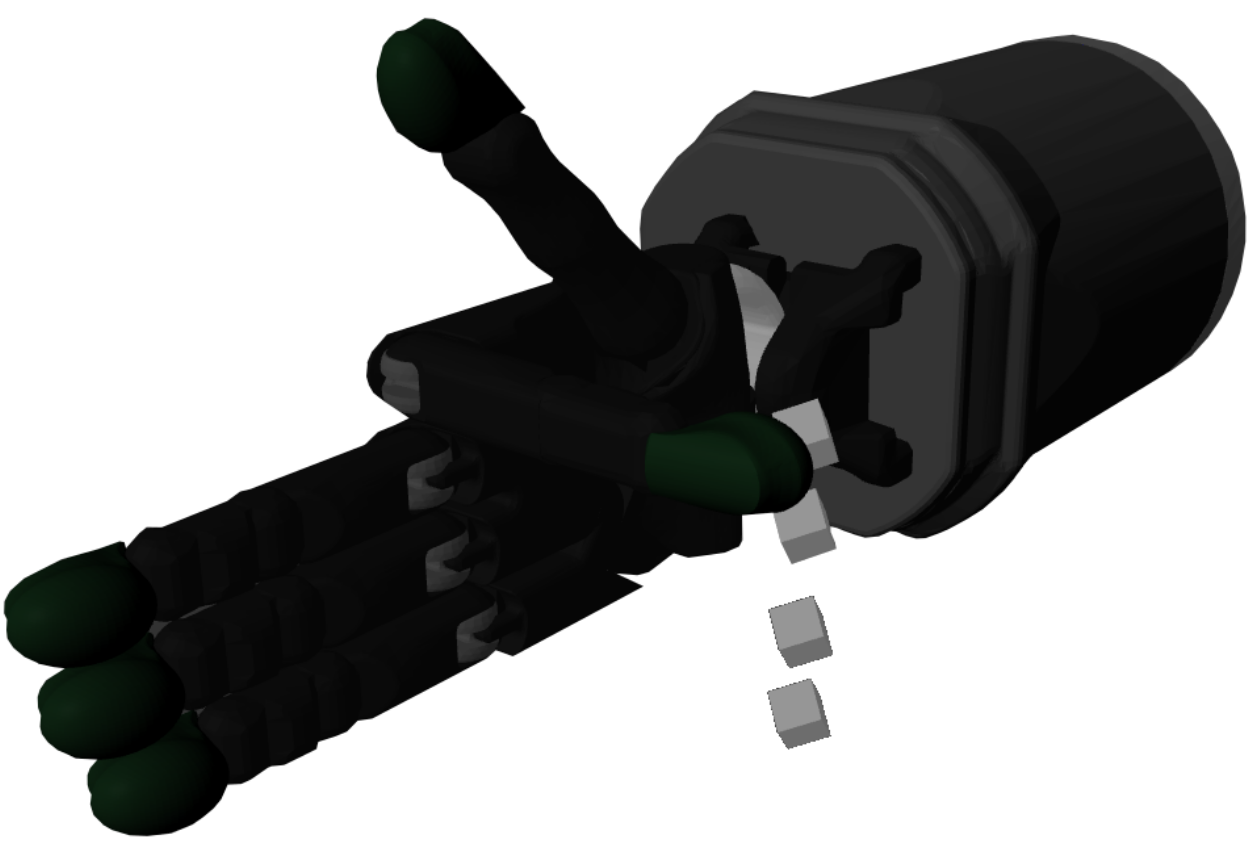
\includegraphics[width=\textwidth]{chapters/1-tactile-perception/fig/experimental-setup/corner-contact.png}
		\caption{Simulated index finger in contact with a corner}
		\label{fig:corner-contact-experimental}
	\end{subfigure}
		\caption{The simulated Shadow Dexterous hand in contact with the four surfaces used to test the performance of the \gls{dl} model's ability to represent surfaces. In each case, the contact is made by the index finger.}
		\label{fig:experimental-setup-tactile-perception-experimental}
\end{figure}

When contact is made the inputs and outputs of the \gls{dl} model are recorded over \SI{30}{\second}, which with a sampling frequency of \SI{100}{\hertz} results in \num{3000} samples. As inputs are collected, the contact positions and forces are given by Gazebo in \robframe{W}, which then is transformed into the contact frame \robframe{C} using the grasping matrix \mat{G}, to ensure consistency. Due to contact data in Gazebo being prone to noise, an exponential decay filter is additionally applied.

% ground truth vectors presented on figures and how errors were computed

% holding bunny, and logging forces. Forces compared to the theoretical ideal.

% as a solution, one can train an object detection NN for converting tactile data into contact points and normals.

\section{Results}\label{sec:1-tactile-perception-results}



After executing the \gls{dl} model on all cases, the resulting simulated electrode activations were discovered to be infinite. Consequently, efforts were undertaken to address this issue. It was determined that the model does not include layer-wise normalization to establish limits on feature responses. The addition of this normalization procedure resulted in the network outputting values within the expected range.~\figref{fig:simulated-electrode-distribution} shows a 3D plot of the electrode activations, while~\figref{fig:electrode-map} shows a 2D projection of the finger tip with its labeled electrodes.

\begin{figure}[h]
	\centering
	\begin{subfigure}[b]{0.48\textwidth}
		\centering
		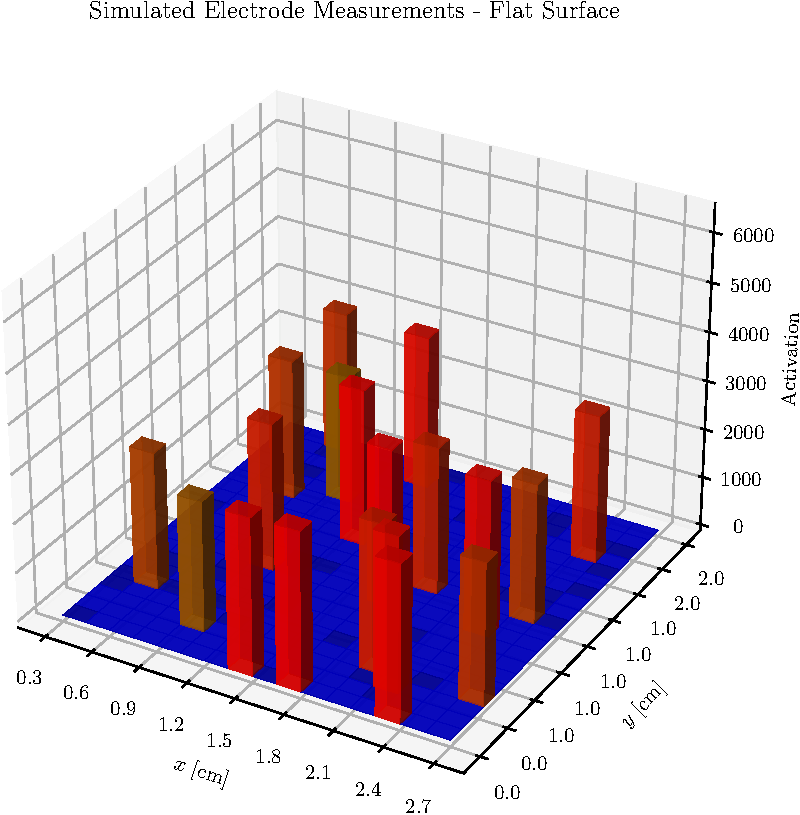
\includegraphics[width=\textwidth]{chapters/1-tactile-perception/fig/pressure-distribution-crop.pdf}
		\caption{3D plot of electrode activations when the Shadow Dexterous hand's index finger makes contact with a flat surface.}
		\label{fig:simulated-electrode-distribution}
	\end{subfigure}
	\hfill
	\begin{subfigure}[b]{0.48\textwidth}
		\centering
		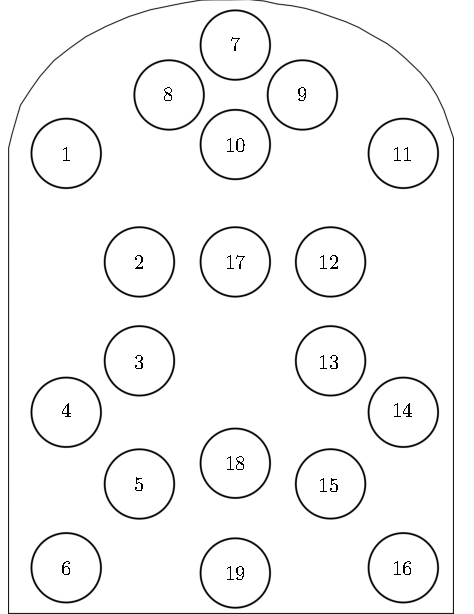
\includegraphics[height=\textwidth]{chapters/1-tactile-perception/fig/electrode-map.pdf}
		\caption{Map showing a 2D projection of the electrodes' positions and numbers.}
		\label{fig:electrode-map}
	\end{subfigure}
		\caption{3D plot of electrode activations and 2D electrode map with labels.}
		\label{fig:flat-contact-experimental-and-electrode-map}
\end{figure}

\figref{fig:flat-contact-graph} illustrates the inputs and outputs of the \gls{dl} model when the Shadow Dexterous hand's index finger makes contact with a flat surface. As seen here, the output of the model is independent from the input. To verify this behavior, data from the data set on which the model has been trained is applied and a similar result is found as seen in~\figref{fig:train-contact-graph}.

\begin{figure}[h]
	\begin{center}
		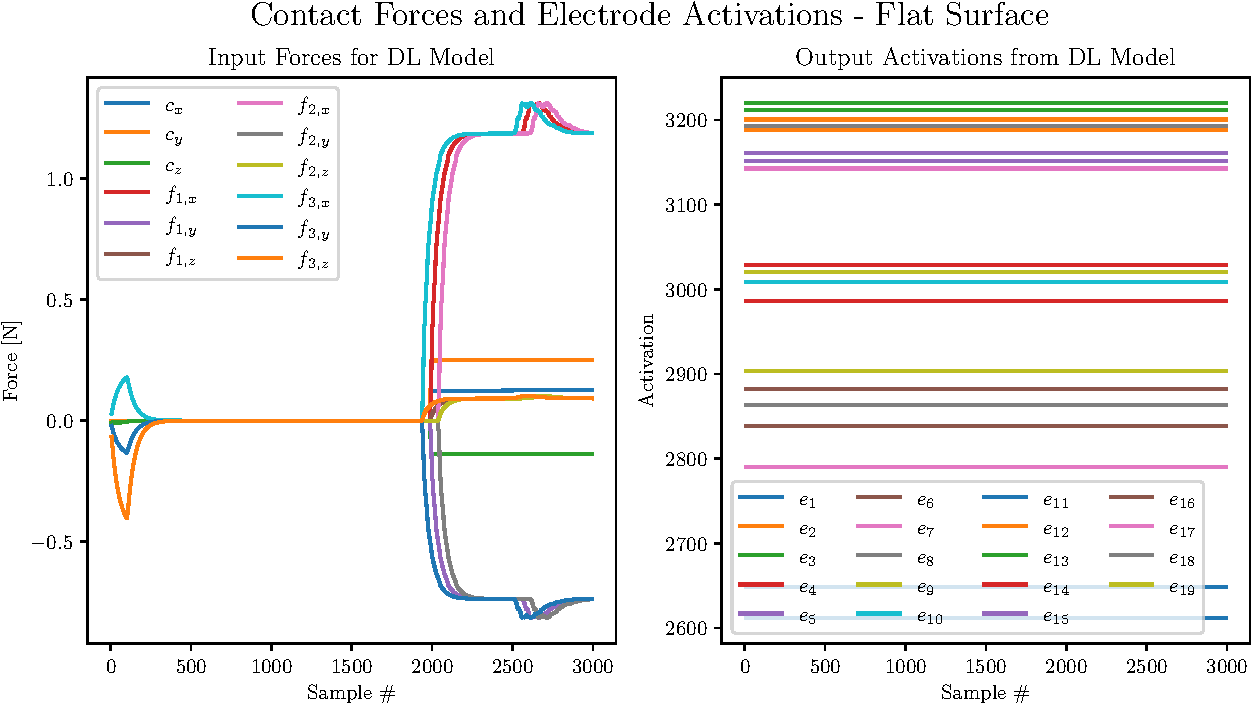
\includegraphics[width=0.85\textwidth]{chapters/1-tactile-perception/fig/flat-contact-graph-crop.pdf}
	\end{center}
	\caption{The simulated tactile electrode activations.}
	\label{fig:flat-contact-graph}
\end{figure}

\begin{figure}[h]
	\begin{center}
		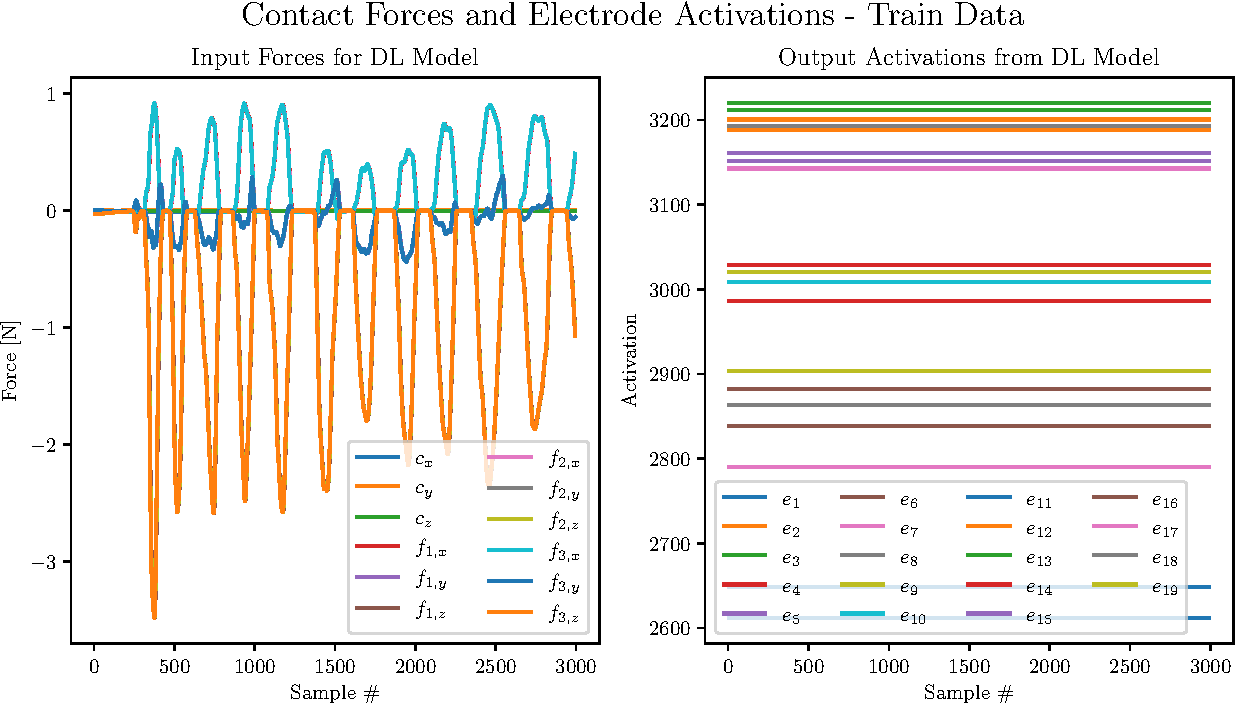
\includegraphics[width=0.825\textwidth]{chapters/1-tactile-perception/fig/train-contact-graph.pdf}
	\end{center}
	\caption{The simulated tactile electrode activations.}
	\label{fig:train-contact-graph}
\end{figure}

Due to this independence of input, the electrodes, and by extension the \gls{dl} model is not judged to be able to accurately simulate skew forces for a BioTac sensor in contact. Instead the linear velocity of contact points

The surface normals can be estimated using recursive least squares to compute the normals based on the linear velocities. The constraints computed can be seen below. \medskip

\begin{equation} \label{eq:recursive-least-squares}
	RLS
\end{equation}

The equation we wish to solve is

\begin{equation} \label{eq:velocity-normal-constraint}
	\vec{v}^\T\vec{n}=0
\end{equation}


based on these results, it can be seen that no valuable information can be derived, and thus to continue the contact information generated by the Gazebo physics engine is used. The data of which will now be presented.

show torques, forces and normals in grid plot.

normal cone and mirrroring error. How it was solved

What is the error.

\section{Discussion \& Conclusion}\label{sec:1-tactile-perception-discussion-and-conclusion}

It seems to represent the real phenomenons realistically 


% \section{Related Work} \label{sec:1-tactile-perception-related-work}

% Here we cite the related work by \texttt{\textbackslash cite\{source-label\}} like this \cite{recent-progress-in-technologies-for-tactile-sensors}